\documentclass[11pt]{article} 
\usepackage{graphicx}
\usepackage{textcomp, gensymb}
\usepackage{amssymb}
\usepackage{enumitem}
\begin{document}

\title{Geometry}
\author{Gnana Sri  Y}
\maketitle

\begin{enumerate}
	\item The angle of elevation of the top of a tower from a point on the ground,which is $30$ m away from the foot of the tower is $45\degree$ .What is the height of the tower ?
	\item Find the sun's altitude if the shadow of a 15 m high tower is ${15}\sqrt{3}$ m.
	\item A circular piece of land is $40$ m in diameter. A well of diameter $16$ m has been dug to a depth of $28$ m and the earth taken out has been spread evenly over the remaining area. How much has the level of ground been raised ?
	\item From a point on the ground, $20$ m away from the foot of vertical tower, the angle of elevation of the top of the tower is $60\degree$. Find the height of the tower.
	\item
	\begin{enumerate}
		\item In a right triangle $ABC$, right-angled at $B$, $BC= 6 cm$ and $AB = 8 cm$. A circle is inscribed in the ${\triangle} ABC$. Find the radius of the incircle.
		\item Two cricles touch externally at $P$ and $AB$ is a common tangent, touching one circle at $A$ and the other at $B$. Find the measure of $\angle APB$.
	\end{enumerate}
	\item A solid sphere of radius $r$ is melted and cast into the shape of a solid cone of height $r$. What is the radius of the base of the cone in terms of $r$ ?
	\item Answer any four of the following questions :
		\begin{enumerate}[label=(\roman*)]
			\item $ABC$ and $BDE$ are two equilateral triangles such that $D$ is the mid-point of $BC$. The ratio of the areas of the triangles $ABC$ and $BDE$ is
				\begin{enumerate}[label=(\Alph*)]
					\item $2 : 1$
					\item $1 : 2$
					\item $4 : 1$
					\item $1 : 4$
				\end{enumerate}
			\item In $\triangle$ $ABC$, $AB = {4\sqrt{3}}$ cm, $AC = 8 cm$ and $BC = 4 cm$. The angle $B$ is
				\begin{enumerate}[label=(\Alph*)]
					\item $120\degree$
					\item $90\degree$
					\item $60\degree$
					\item $45\degree$
				\end{enumerate}
			\item The perimeters of two similar triangles are $35 cm$ and $21 cm$ respectively. If one side of the first triangle is  $9 cm$,then the corresponding side of the second triangle is
				\begin{enumerate}[label=(\Alph*)]
					\item $5.4 cm$
					\item $4.5 cm$
					\item $5.6 cm$
					\item $15 cm$
				\end{enumerate}
			\item In a $\triangle$ $ABC, D$ and $E$ are points on the sides $AB$ and $AC$ respectively such that $DE || BC$ and $AD : DB = 3 : 1$. If $AE = 3.3 cm$,then AC is equal to
				\begin{enumerate}[label=(\Alph*)]
					\item $4 cm$
					\item $1.1 cm$
					\item $4.4 cm$
					\item $5.5 cm$
				\end{enumerate}
			\item In an isosceles triangle $ABC$, if $AC = BC$ and ${AB}^2 = 2{AC}^2$, then $\angle C$ is equal to
				\begin{enumerate}[label=(\Alph*)]
					\item $30\degree$
					\item $45\degree$
					\item $60\degree$
					\item $90\degree$
				\end{enumerate}

		\end{enumerate}
	\item To explain how trignometry can be used measure the height of an inaccessible object, a teacher gave the following example to students :

		A TV tower stands vertically n the bank of a canal. From a point on the other bank direct opposite the tower, the angle of the elevation of the top of the tower is $60\degree$.From another point 20 m away from this point to the foot of the tower, the angle of elevation of the top of the tower is $30\degree$ (as shown in Figure 1).

		\begin{figure}[ht!]
			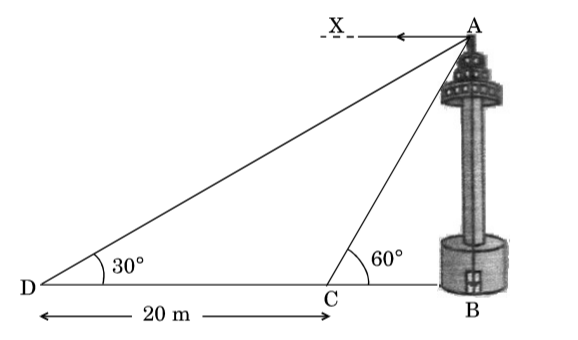
\includegraphics[width=\columnwidth]{Figs/Problem.png}
			\caption{Projection of Tower}
			\label{fig:traingle}
		\end{figure}
		Based on the above, answer the following questions :
		\begin{enumerate}[label=(\roman*)]
			\item The width of the canal is
				\begin{enumerate}[label=(\Alph*)]
					\item ${10}\sqrt{3} m$
					\item ${20}\sqrt{3} m$
					\item $10 m$
					\item $20 m$
				\end{enumerate}
			\item Height of the tower is
				\begin{enumerate}[label=(\Alph*)]
					\item ${10}\sqrt{3} m$
					\item $10 m$
					\item ${20}\sqrt{3} m$
					\item $20 m$
				\end{enumerate}
			\item Distance of the foot of the tower from the point $D$ is
				\begin{enumerate}[label=(\Alph*)]
					\item $20 m$
					\item $30 m$
					\item $10 m$
					\item ${20}\sqrt{3} m$
				\end{enumerate}
			\item The angle formed by the line of sight with the horizontal when it is above the horizontal line is known as
				\begin{enumerate}[label=(\Alph*)]
					\item angle of depression
					\item line of sight
					\item angle of elevation
					\item obtuse angle
				\end{enumerate}
			\item In above figure, measure of angle $XAC$ is
				\begin{enumerate}[label=(\Alph*)]
					\item $30\degree$
					\item $60\degree$
					\item $90\degree$
					\item $45\degree$
				\end{enumerate}
		\end{enumerate}
	\item A children's park is in the triangular shape as shown in the below figure.In the middle of the park, there is a circular region for younger children to play. It is fenced with three layers of wire. The radius of the circular region is $3 m$.
		\begin{figure}[ht!]
		\centering
		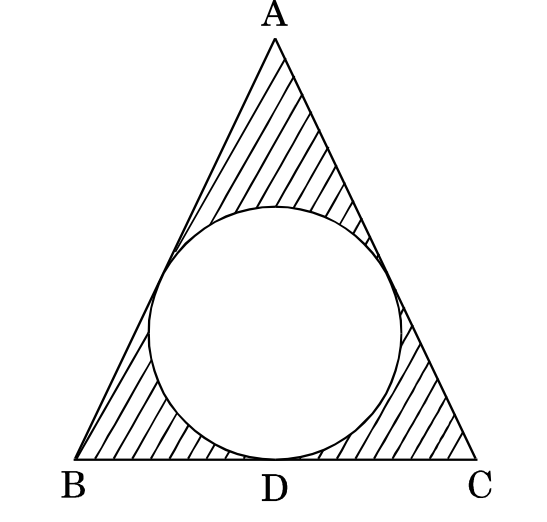
\includegraphics[width=\columnwidth]{Figs/Park.png}
		\caption{Children's Park in triangular shape}
		\label{fig:Park}
		\end{figure}
		Based on the above,answer the following questions:
		\begin{enumerate}[label=(\roman*)]
			\item The perimeter(or circumference) of the circular region is
				\begin{enumerate}[label=(\Alph*)]
					\item $3\pi m$
					\item ${18}\pi m$
					\item $6\pi m$
					\item $9\pi m$
				\end{enumerate}
			\item The Total length of wire used is
				\begin{enumerate}[label=(\Alph*)]
					\item $9\pi m$
					\item ${18}\pi m$
					\item ${54}\pi m$
					\item ${27}\pi m$
				\end{enumerate}
			\item The area of the circular region is
				\begin{enumerate}[label=(\Alph*)]
					\item ${54}\pi m^2$
					\item ${3}\pi m^2$
					\item ${18}\pi m^2$
					\item ${9}\pi m^2$
				\end{enumerate}
			\item If $BD = 6 m$, $DC = 9 m$ and ar ($\triangle ABC = 54$ $m^2$,then the length of sides $AB$ and $AC$, respectively, are)
				\begin{enumerate}[label=(\Alph*)]
					\item $9 m, 12 m$
					\item $12 m, 9 m$
					\item $10 m, 12 m$
					\item $12 m, 10 m$
				\end{enumerate}
			\item The perimter of $\triangle ABC$ is
				\begin{enumerate}[label=(\Alph*)]
					\item $28 m$
					\item $37 m$
					\item $36 m$
					\item $38 m$
				\end{enumerate}
		\end{enumerate}		
\end{enumerate}

\end{document}
